Большинство программных систем, имеющих сложную структуру и состоящих из
нескольких сотен различных компонент, обладают рядом схожих проблем.
Например веб-поиск содержит следующие компоненты:
балансеры, верхние, средние метапоиски, промежуточные и базовые поиски,
колдунщики, антироботы, свежесть, региональные поиск,
несколько десятков параллельных поисков.
% Краткое схематичное описание архитектуры:

% 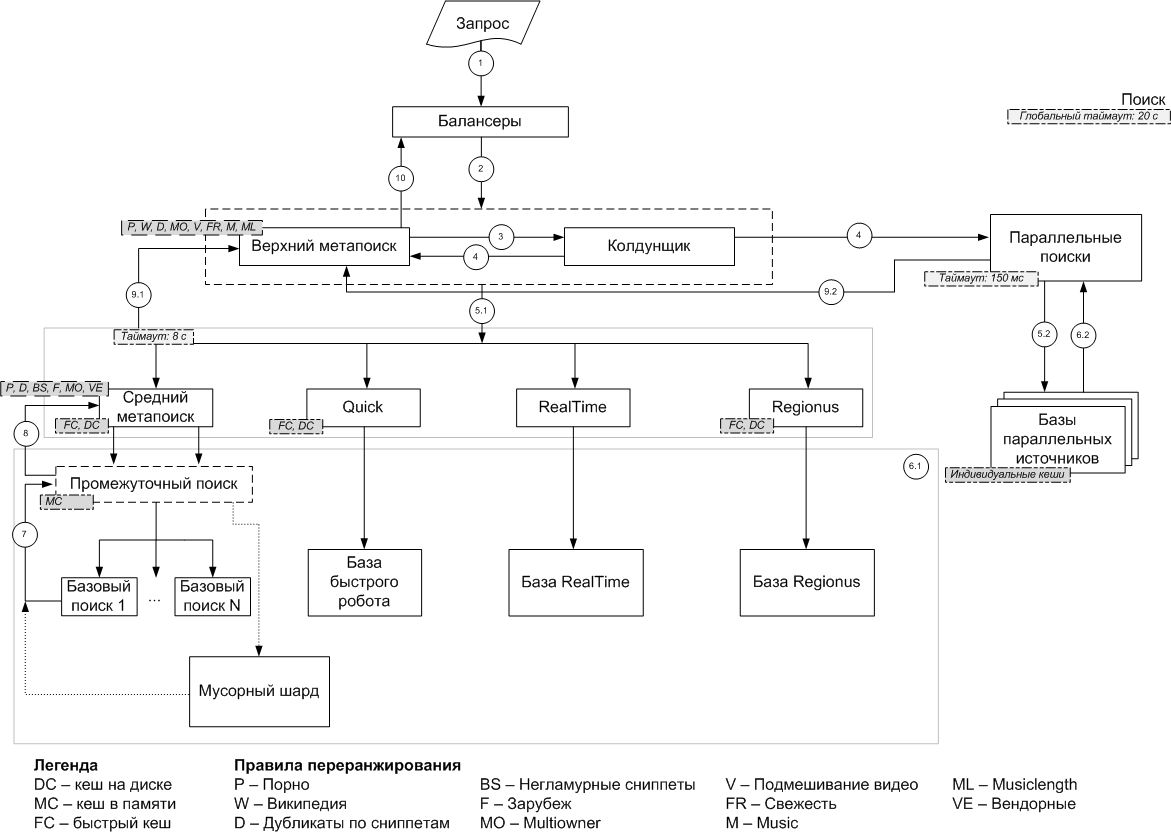
\includegraphics[width=\textwidth]{pics/search.png}

\begin{definition}[Экземпляр]
  приложение, запущенное в контейнере и описываемое парой host:port.
\end{definition}
Всего единовременно запущено несколько ******** тысяч экземпляров приложений.
Каждый экземпляр генерирует множество ошибок и записывает каждую из них в
файл журнала ошибок.

Некоторые приложения, близкие по функционалу, пишут в один и тот же файл.
Файлы журналов ротируются согласно определённому алгоритму. Тем не менее объем
файла журнала для одного экземпляра может достигать нескольких сотен мегабайт,
что препятствует быстрому ручному анализу в случае инцидента и инженеры
вынуждены тратить ценные секунды на просмотр сотен тысяч строк файла в поисках
сообщения с описанием элемента, вызвавшего сбой работы системы.

Начальным требованием к системе для эффективного использования алгоритма
является наличие сопоставимого с количеством поисковых экземпляров
приложений количества узлов на которых может быть запущена программа,
реализующая алгоритм.

В организации, в которой выполнялась учебно-исследовательская работа,
развёрнута большая поисковая инфраструктура, которая не лишена недостатков и
существует вероятность поломки некоторой её части. Существует множество
средств мониторинга состояния веб-поиска и противодействия инцидентам,
но в некоторых случаях инженерам их недостаточно и приходится вручную
анализировать файлы журналов отдельных экземпляров приложений на отдельных
сервераз, что, в свою очередь, замедляет скорость реакции на непредвиденную
ситуацию. Но даже автоматизация процесса анализа файла журнала одного
экземпляра не решает проблему полностью, поэтому необходима возможность
быстрого анализа файлов журналов сразу множества экземпляров.

\begin{definition}[Шаблон]
  Специально подготовленное регулярное выбражение с экранированными
  спецсимволами.
\end{definition}
Таким образом, целью этой учебно-исследовательской работы является разработка
алгоритма, позволяющего собирать статистику по ошибкам, встречающимся
в файлах журналов экземпляров поисковых приложений на основе существующих
шаблонов и выделять новые шаблоны.
